\section{Preliminaries} 
\label{sec:Prelim} 

Our proposal, \dyntset, relies mainly on three structures, a \textit{monoid}, a \textit{set} and a \textit{finger tree}, which are briefly described in the following subsections. 

\subsection{Monoid}

A \textit{monoid} is a triple $(S,\star,e)$, where $S$ is a set, $\star$ is a binary operation, called $product$ and $e$ is an element of $S$, called $unit$, satisfying the following properties:

\begin{enumerate}
\item $e \star x = x = x \star e$, for all $x \in S$ 
\item $x \star (y \star z) = (x \star y) \star z $, for all $x,y,z \in S$.  
\end{enumerate}

The type class Haskell implementation of a monoid we have:
%\begin{verbatim}
\begin{lstlisting}[mathescape]
class Monoid  a where 
   mempty  :: a
   mappend :: a $\to$ a $\to$ a
\end{lstlisting}   
%\end{verbatim}

where the function \code{mempty} represents the element $e$ and the function \code{mappend} represents function $\star$. Detailed information about monoids within the functional programming can be found in \cite{Monoids}, and for the Haskell implementation at \cite{HaskellMonoid}.


\subsection{Set as binary search tree} 

A set, as a data structure, is used here for searching purposes, seen as testing membership within a specific set. Also, we look for incorporating elements into a set in order to increase such set for further look ups. This incorporation, comes in two flavours, either as single insertion or as the set-union operation. Finally, the presence of an empty set, a set with no elements at all, is crucial since it is the $unit$ when a set behaves as monoid. Also, an empty set is a starting point when a forest contains no trees.

Internally, a set is implemented as binary search tree, also called BST. A BST is either a \textit{leaf} (also called a \code{tip}) or a vertex consisting of a \textit{value}, a \textit{left} BST and a \textit{right} BST. The height of the tree determines the time taken to perform every operation onto it, therefore the shorter the height the better, and this is done throughout a \textit{balancing scheme}. The study of BSTs is vast and there are several implementation around. In our case, a \textit{size balanced} and a \textit{pairing hashed} are used. A detailed comparison and benchmarking is outside the scope of the present work.

The following is an snippet of \code{Data.Set} \footnote{https://hackage.haskell.org/package/containers-0.5.10.2/docs/Data-Set.html}
%\begin{verbatim}
\begin{lstlisting}
data Set a    = Bin Size a (Set a) (Set a)
              | Tip
\end{lstlisting}              
%\end{verbatim}

In Table~\ref{tab:Setfuncs} we show the set-functions we have incorporated in \code{dynTsET} from \code{Data.Set}.
\small
\begin{table}[H]
\begin{center}
\begin{tabular}{||l | l | c||} 
 \hline
 Function         & Type                                   & Time complexity            \\ 
 \hline\hline
 \texttt{empty}   & \texttt{Set a}                         & $O(1)$                     \\ 
 \hline
 \texttt{insert}  & \texttt{a $\to$ Set a $\to$ Set a}     & $O(\log n)$                \\
 \hline
 \texttt{member}  & \texttt{a $\to$ Set a $\to$ Bool}      & $O(\log n)$                \\ 
 \hline
 \texttt{union}   & \texttt{Set a $\to$ Set a $\to$ Set a} & $O(m(\log\frac{n}{m} +1))$ \\
 \hline
\end{tabular}
\caption{Leijen's implementation of \code{Data.Set} \cite{HaskellSet}, based on \cite{ParallelSets}}
\label{tab:Setfuncs} 
\end{center}
where $n$ and $m$ are the sizes of the largest and smallest sets respectively
\end{table}
\normalsize

Functions \code{empty} and \code{union} are, in fact, the monoidal functions \code{mempty} and \code{mappend} respectively. 

\subsection{Euler-tour tree} 
\label{sec:ETt}
Dealing with trees of different degree can be complicated. A simple way to handle and represent trees of any degree is by an Euler tour, that is, a sequence as in \cite{Rand-DynGs-Algos} and \cite{WerneckR-PhD}. To represent a tree $t$, we replace every edge $\langle u,v \rangle$ of $t$ by two arcs $(u,v)$ and $(v,u)$, and add a loop $(v,v)$ to represent each vertex $v$. In this context, a tree $t$ can have at least one, and in general, many Euler tours. The size of an Euler tour \textit{et} of $t$ is $et(t) = v + 2e $, where $v$ is the number of vertices of $t$ and $e$ its number of edges. We can represent an Euler tour in Haskell simply as a list of pairs, such in 

%\begin{verbatim}
\begin{lstlisting}
data EulerTour a = [(a,a)] 
\end{lstlisting}
%\end{verbatim}

By managing the tour with lists, we can perform insertion from the left (head) in $O(1)$ but remaining operations such insertion from the right, access, cutting, appending and inserting might take $O(n)$ per operation.
On the other hand, representing tours through finger trees, performance per operation is improved up to $O(\log n)$ per operation amortised as we explain shortly and in Section~\ref{sec:TechDes}. 

Our representation of $k$-trees through Euler-tour will not close up the tour with the first node as this avoids the uniqueness presence for such a node, as shown in Fig.~\ref{fig:Euler-tour}.

\begin{figure}[H]
\begin{center}
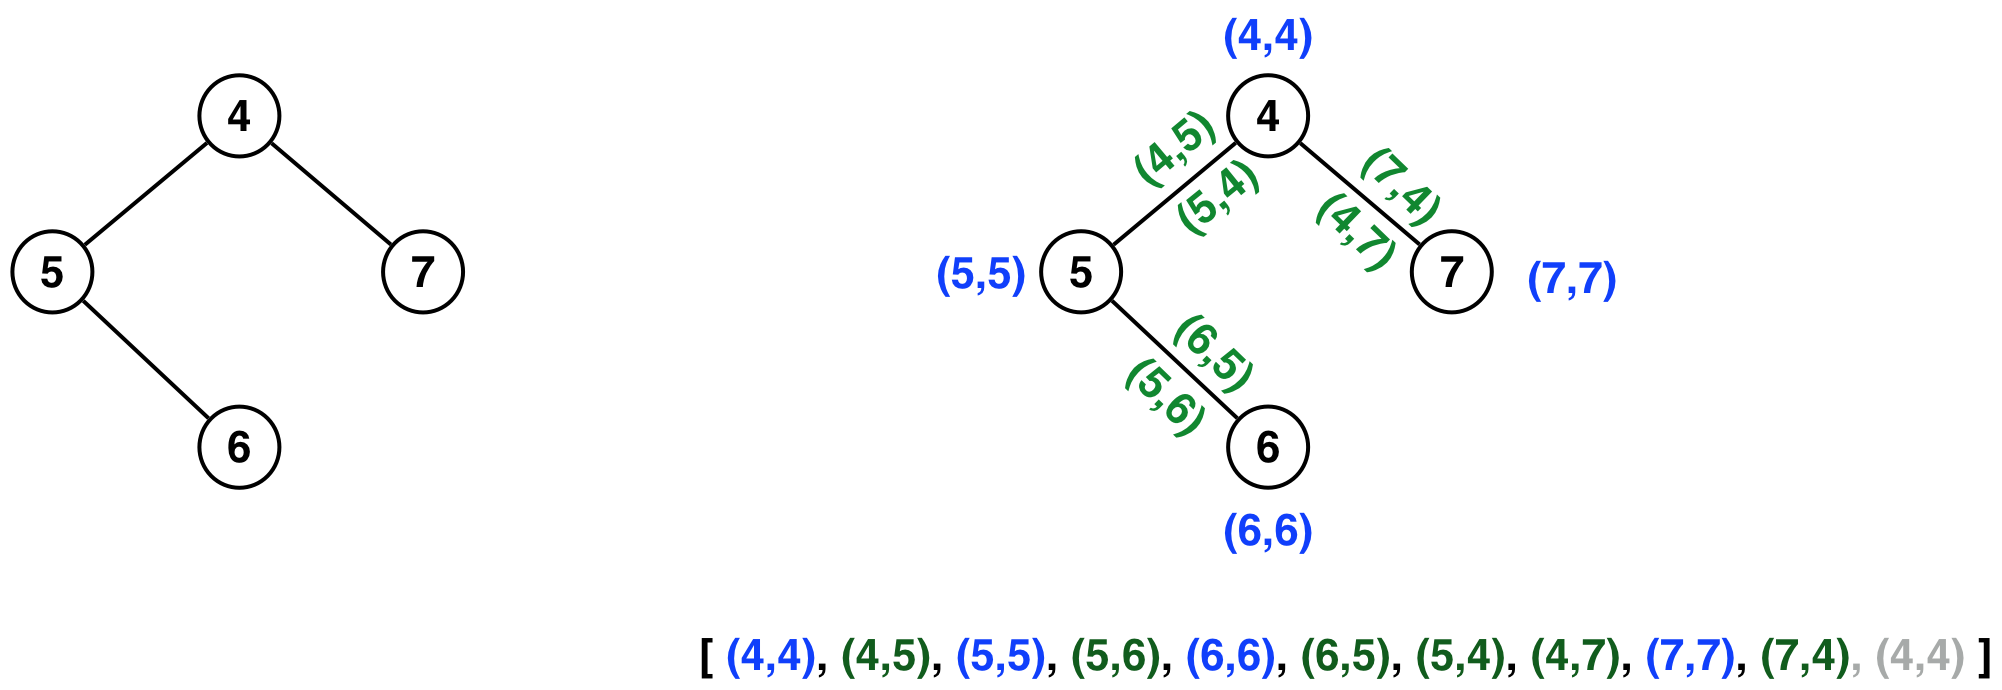
\includegraphics[scale=0.35]{./Images/Euler-tour} 
\end{center}
\caption{The $k$-tree (left) is represented as a sequence of size $v+2e$ (right). Notice we left out the final node-pair to preserve uniqueness}
\label{fig:Euler-tour}
\end{figure}


\subsection{Finger tree} 

We present Hinze and Paterson's version of finger trees \madd{(FTs)} \cite{FTs}. A finger tree is a 2-3-4 tree data structure which is always balanced. The structure is designed to store the elements of a sequence in the terminal nodes or leaves while intermediate nodes are dedicated for monoidal annotations. These annotations help out to achieve a specific task when storing or retrieving values in the leaves or when dealing with the tree itself such concatenation or splitting. One instance is random-access on lists. In order to speed up the time taken by a list for accessing the $n$th element, a finger tree stores the list elements on its leaves and the type \code{Sum Int} as its monoidal annotation. In this way, we can ask for a specific element provided its index in $O(\log n)$ rather than $O(n)$ time. This done through monoidal instances for \code{Sum}. The identity is defined as zero as in 
\begin{lstlisting}[mathescape]
instance Num a $\Rightarrow$ Monoid (Sum a) where
        mempty = Sum 0
\end{lstlisting}

and the corresponding binary operation on integers which preserves its identity (arithmetic addition),
\begin{lstlisting}[mathescape]
instance Num a $\Rightarrow$ Semigroup (Sum a) where
        (<>) = coerce ((+) :: a $\to$ a $\to$ a)
\end{lstlisting}


The finger tree data type in Haskell is defined as

\begin{figure}[H]
\begin{lstlisting}
data FingerTree v a = Empty
                    | Single a 
                    | Deep v 
                           Digit a 
                           FingerTree v (Node v a) 
                           Digit a
\end{lstlisting}                           
\caption{Data type of the finger tree by Hinze and Paterson}
\label{fig:FTdatatype}
\end{figure}

\code{Digit} type holds from one up to four elements of type \code{a}. \code{Node} type can hold two or three elements of type \code{a}. The recursive and nested definition of \code{FingerTree} forces the structure to be balanced by its types, instead of enforcing it by code invariants. In our case, the leaves of a finger tree stores pairs of nodes or vertices representing an Euler tour. To implement \textit{updates} and \textit{lookups} efficiently, Hinze and Paterson \cite{FTs} added a monoidal annotation on the intermediate vertices, the \code {v} type.

In Fig.~\ref{fig:FT-Euler-tour} we can see our example of the Euler-tour sequence in Fig.~\ref{fig:Euler-tour} managed by the data constructors described above.

\begin{figure}[H]
\begin{center}
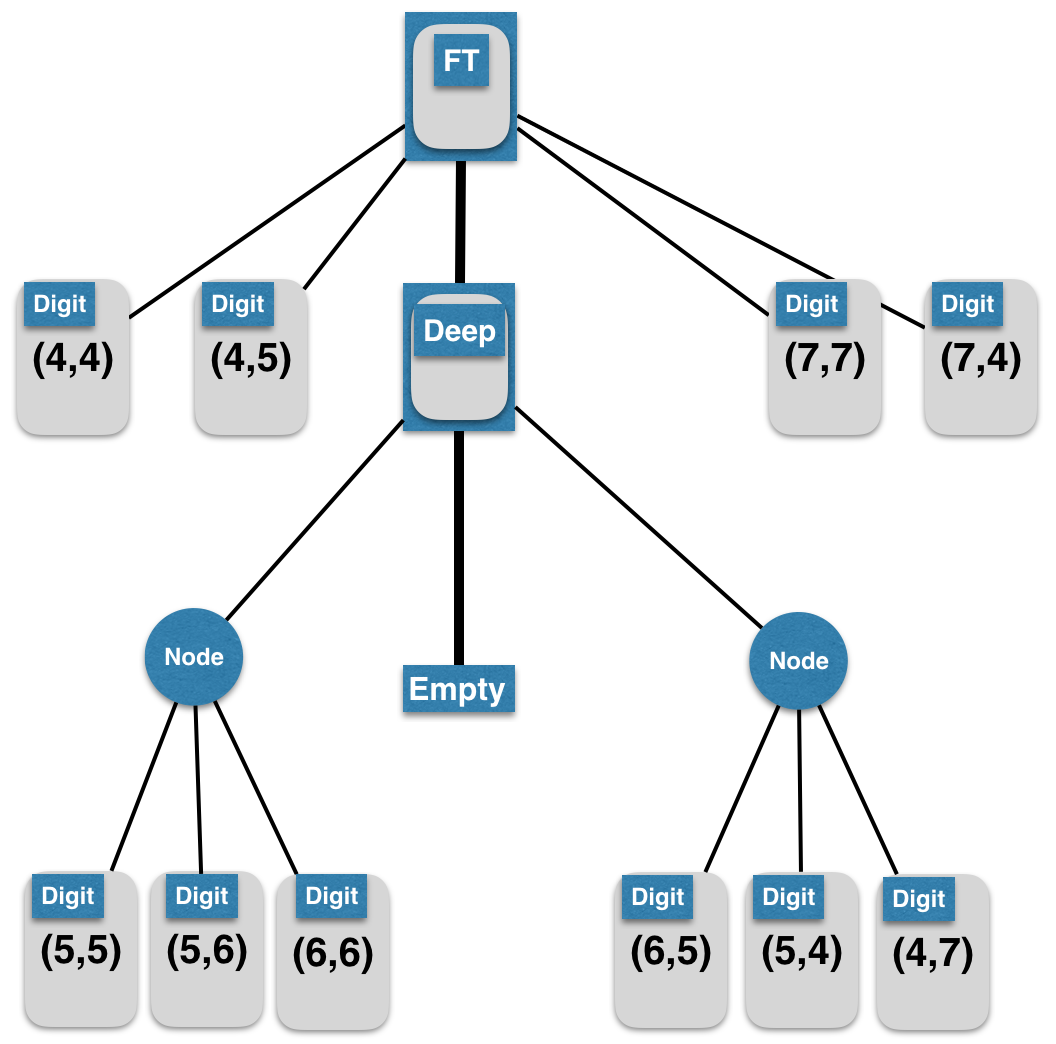
\includegraphics[scale=0.35]{./Images/FT-Euler-tour} 
\end{center}
\caption{A finger tree (FT) holding the sequence (Euler-tour) that represents the $k$-tree in Fig.\ref{fig:Euler-tour}}
\label{fig:FT-Euler-tour}
\end{figure}

Since the backbone of our structure \dyntset is actually a Hinze's and Paterson finger tree \cite{FTs}, we show the functions involved in our proposal, those to deal with inserting, cutting, appending and accessing finger trees. There are plenty of additional functions from finger trees we do not cover and that can be reached at \url{http://hackage.haskell.org/package/fingertree-0.1.4.1/docs/Data-FingerTree.html}.

\small
\begin{table}[H]
\begin{center}
\begin{tabular}{||l | l | c||} 
 \hline
 Function         & Type                                   & 
      \begin{tabular}{c} Time complexity \\ 
                         (amortised bounds)
      \end{tabular} \\
 \hline\hline
 \texttt{viewl}   & 
      \begin{tabular}{l} \texttt{FingerTree v a}   \\ 
                         \texttt{$\to$ ViewL (FingerTree v a)  } 
      \end{tabular}
                  & $O(1)$ \\ 
 \hline
 \texttt{search}  & 
      \begin{tabular}{l} \texttt{(v $\to$ v $\to$ Bool)}   \\ 
                         \texttt{$\to$ FingerTree v a  }   \\ 
                         \texttt{$\to$ SearchResult v a  } 
      \end{tabular}
          & $O(\log(min(i,n-i)))$  \\ 
 \hline
 \texttt{$\lhd$} (ins. from left) & 
      \begin{tabular}{l} \texttt{a $\to$ FingerTree v a} \\
                         \texttt{$\to$ FingerTree v a} 
      \end{tabular}
          & $O(1)$                \\
 \hline
 \texttt{$\rhd$} (ins. from right) & 
      \begin{tabular}{l} \texttt{FingerTree v a $\to$ a} \\
                         \texttt{$\to$ FingerTree v a} 
      \end{tabular}
          & $O(1)$                \\
 \hline
 \texttt{$\bowtie$} (concatenation) & 
      \begin{tabular}{l} \texttt{FingerTree v a} \\
                         \texttt{$\to$ FingerTree v a} \\
                         \texttt{$\to$ FingerTree v a} 
      \end{tabular}
          & $O(\log ( min(m,n) ))$         \\
 \hline
\end{tabular}
\caption{Hinze's and Paterson implementation of \code{Data.FingerTree} \cite{FTsURL}, based on \cite{FTs}}
\label{tab:FTfuncs} 
\end{center}
\end{table}
\normalsize

where $n$ is the size of the largest sequence, $m$ is the size of the smaller sequence (i.e. when concatenating) and $i$ is the index of the element when searching. 

\tcb{SPLIT is not longer used, instead there is SEARCHFT, which aim is the same as SPLIT and hope it will be easier to explain}

\tcb{Is it the ``best" part in the document to bring up an explanations or examples or both for amortisation?}